\chapter{Dezvoltarea Aplicației}

Implementarea soluției propuse a implicat dezvoltarea a două componente principale: un API backend robust, responsabil pentru logica de business, procesarea datelor și interacțiunea cu serviciile externe, și o aplicație mobilă cross-platform, care oferă interfața pentru utilizatorul final.

\section{Arhitectura și Dezvoltarea API-ului Backend}

\begin{figure}[h!]
    \centering
    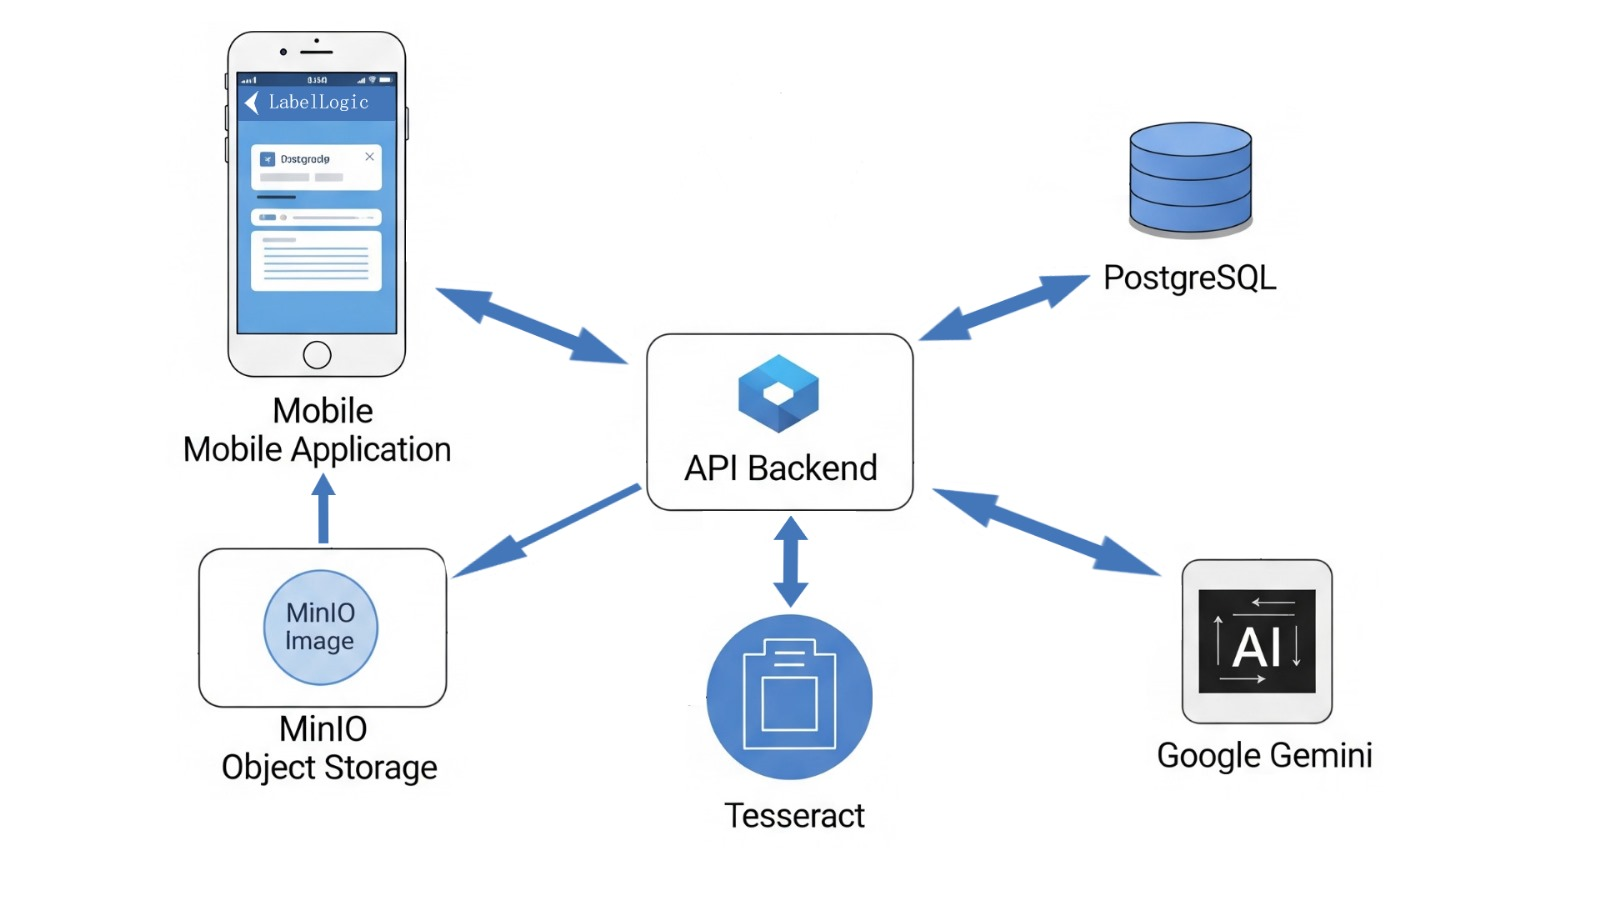
\includegraphics[width=0.9\textwidth]{images/Arhitectura_aplicatiei.jpg}
    \caption{Diagrama arhitecturală a sistemului, ilustrând interacțiunea dintre aplicația mobilă, API-ul backend și serviciile externe.}
    \label{fig:system-architecture}
\end{figure}

Componenta backend a fost proiectată ca un sistem de microservicii containerizat Figura~\ref{fig:system-architecture}, o abordare modernă care asigură scalabilitate, mentenabilitate și izolare. S-a optat pentru Docker \cite{Docker} pentru containerizare, orchestrând serviciile prin Docker Compose. Această arhitectură a permis definirea unor medii de dezvoltare și producție consistente și a facilitat integrarea componentelor eterogene: API-ul principal, baza de date și sistemul de stocare a obiectelor.

Ca fundament pentru API, a fost ales framework-ul FastAPI \cite{FastAPI}, recunoscut pentru performanța sa ridicată, suportul nativ pentru operațiuni asincrone și generarea automată de documentație conform standardului OpenAPI. Structura proiectului a fost modularizată, separând endpoint-urile API, modelele de date (folosind SQLAlchemy ORM), serviciile care încapsulează logica de business și modulele de configurare.

\subsection{Servicii de Procesare a Datelor: OCR și AI}

Nucleul funcțional al aplicației constă în capacitatea de a extrage și interpreta automat datele de pe etichetele produselor. Pentru recunoașterea optică a caracterelor (OCR), s-a integrat motorul open-source Tesseract \cite{Tesseract}, configurat specific pentru a gestiona limbile română și engleză.

Pentru etapa de analiză a ingredientelor, s-a realizat o integrare cu API-ul multimodal Google Gemini \cite{GeminiAPI}. Acest serviciu de inteligență artificială procesează atât textul extras prin OCR, cât și imaginea originală, permițând o analiză contextuală superioară. Sistemul a fost proiectat pentru a fi robust, implementând mecanisme de reîncercare cu backoff exponențial în caz de erori tranzitorii. Serviciul AI nu doar că traduce terminologia științifică într-un limbaj accesibil, dar identifică și rolul fiecărui ingredient și calculează un scor de procesare (între 1 și 5), oferind utilizatorului o evaluare rapidă a produsului.

Dat fiind timpul considerabil necesar pentru procesarea OCR și AI (peste 3 secunde), aceste operațiuni au fost implementate ca sarcini asincrone (background tasks). Această abordare decuplată permite API-ului să răspundă instantaneu la cererea de încărcare a imaginilor, în timp ce procesarea rulează în fundal. Progresul este urmărit printr-un sistem de stări detaliat (\texttt{processing}, \texttt{analyzing\_nutrition}, \texttt{completed}, \texttt{error}), pe care aplicația mobilă îl poate interoga pentru a oferi feedback în timp real utilizatorului.

\subsection{Sistemul de Autentificare și Stocare a Fișierelor}

Securitatea și managementul utilizatorilor sunt asigurate printr-un sistem de autentificare bazat pe standardul JSON Web Tokens (JWT) \cite{JWT}. S-a implementat o strategie cu token-uri duale: un \textit{access token} cu durată scurtă de viață pentru autorizarea cererilor și un \textit{refresh token} cu durată lungă pentru reînnoirea sesiunii. Pentru a contracara atacurile de tip Cross-Site Scripting (XSS), token-urile sunt stocate în cookie-uri setate cu atributul \texttt{HttpOnly}, prevenind astfel accesul din JavaScript. Pentru integrarea cu aplicația mobilă, s-a implementat și transmiterea token-urilor in response-uri, asigurând astfel că aplicația le va putea stoca în mod securizat. Sistemul include funcționalități complete pentru înregistrare, validare prin e-mail, autentificare și revocare granulară a sesiunilor.

Pentru stocarea imaginilor încărcate de utilizatori, s-a optat pentru MinIO \cite{MinIO}, o soluție de stocare de obiecte high-performance, compatibilă cu API-ul Amazon S3. Această alegere oferă scalabilitate și flexibilitate. Accesul la fișiere este strict controlat prin generarea de URL-uri pre-semnate cu o durată de viață limitată, asigurând că un utilizator poate accesa doar resursele care îi aparțin.

\section{Dezvoltarea Aplicației Mobile}

Aplicația mobilă a fost dezvoltată folosind React Native \cite{ReactNative} și platforma Expo \cite{Expo}. Această combinație tehnologică a fost aleasă pentru a permite dezvoltarea rapidă a unei aplicații cross-platform (iOS și Android) dintr-o singură bază de cod, beneficiind în același timp de un ecosistem bogat de unelte și servicii care simplifică procesul de build și deployment.

\subsection{Interfața Utilizator și Funcționalități Principale}

Fluxul de autentificare a fost proiectat pentru o experiență mobilă fluidă, cu ecrane dedicate pentru înregistrare și login. Token-urile de autentificare sunt stocate în mod securizat pe dispozitiv folosind funcționalitățile native oferite de Expo, asigurând persistența sesiunii între utilizări.

Ecranul principal al aplicației prezintă lista de alimente adăugate de utilizator, implementată cu tehnici de optimizare precum paginarea (lazy loading) pentru a asigura performanțe ridicate chiar și în cazul listelor lungi. Fiecare element din listă afișează informații esențiale, inclusiv un indicator vizual al stării de procesare și scorul de procesare, colorat corespunzător pentru o identificare rapidă.

Procesul de adăugare a unui nou aliment este facilitat de integrarea cu camera dispozitivului și galeria foto, folosind unelte din ecosistemul Expo. Utilizatorul poate previzualiza imaginile înainte de a le încărca, iar interfața oferă feedback vizual pe durata transferului către server.

Ecranul de detalii constituie piesa centrală a experienței, unde utilizatorul poate vizualiza rezultatele complete ale analizei. Aici sunt afișate informațiile nutriționale într-un format structurat și lizibil, alături de analiza detaliată a ingredientelor generată de AI. Pentru alimentele aflate în curs de procesare, un hook personalizat (\texttt{useProcessingStatus}) interoghează periodic starea de pe server și actualizează automat interfața la finalizarea analizei, fără a necesita intervenția utilizatorului.

\subsection{Managementul Avansat al Datelor}

Aplicația oferă utilizatorilor un control deplin asupra datelor lor. Funcționalitatea de editare permite modificarea numelui, mărcii, sau chiar a textului extras prin OCR, cu posibilitatea de a solicita o nouă analiză AI. De asemenea, utilizatorii pot înlocui imaginile, declanșând o reprocesare completă.

Pentru a spori utilitatea aplicației, au fost implementate funcționalități avansate de filtrare și sortare. Utilizatorii pot filtra lista de alimente pe baza unor criterii multiple, precum conținutul minim de proteine, limita maximă de calorii sau scorul de procesare. Un sistem de ranking permite sortarea listei după diverse atribute nutriționale. În plus, a fost creat un ecran "global" care permite explorarea tuturor alimentelor din baza de date a aplicației, facilitând descoperirea de noi produse și comparația între acestea.

\section{Arhitectura Bazei de Date și Măsuri de Securitate}

Baza de date, implementată pe PostgreSQL, a fost modelată pentru a susține eficient funcționalitățile aplicației, ilustrate în Figura~\ref{fig:db-diagram}. Tabelul \texttt{Users} stochează informațiile de cont, în timp ce tabelul \texttt{Foods} conține toate datele nutriționale, textul brut extras prin OCR, analiza generată de AI, starea de procesare și referințele către imaginile stocate în MinIO. Un tabel separat, \texttt{Tokens}, este dedicat gestionării sesiunilor de autentificare, permițând revocarea acestora și asigurând un nivel înalt de securitate.

Securitatea a fost un pilon central în proiectare. La nivel de backend, parolele sunt securizate folosind algoritmul bcrypt cu salt-uri generate automat. Toate operațiunile asupra datelor impun o validare strictă a proprietarului (ownership), asigurând izolarea completă a datelor între utilizatori. Validarea riguroasă a tuturor datelor de intrare prin Pydantic previne vulnerabilități comune, precum injecțiile SQL. Performanța este asigurată prin paginarea rezultatelor, procesarea asincronă a sarcinilor costisitoare și utilizarea unui pool de conexiuni la baza de date. Un sistem detaliat de logging și monitorizare a fost implementat pentru a urmări operațiunile critice și pentru a facilita depanarea și auditul.

\begin{figure}[h!]
    \centering
    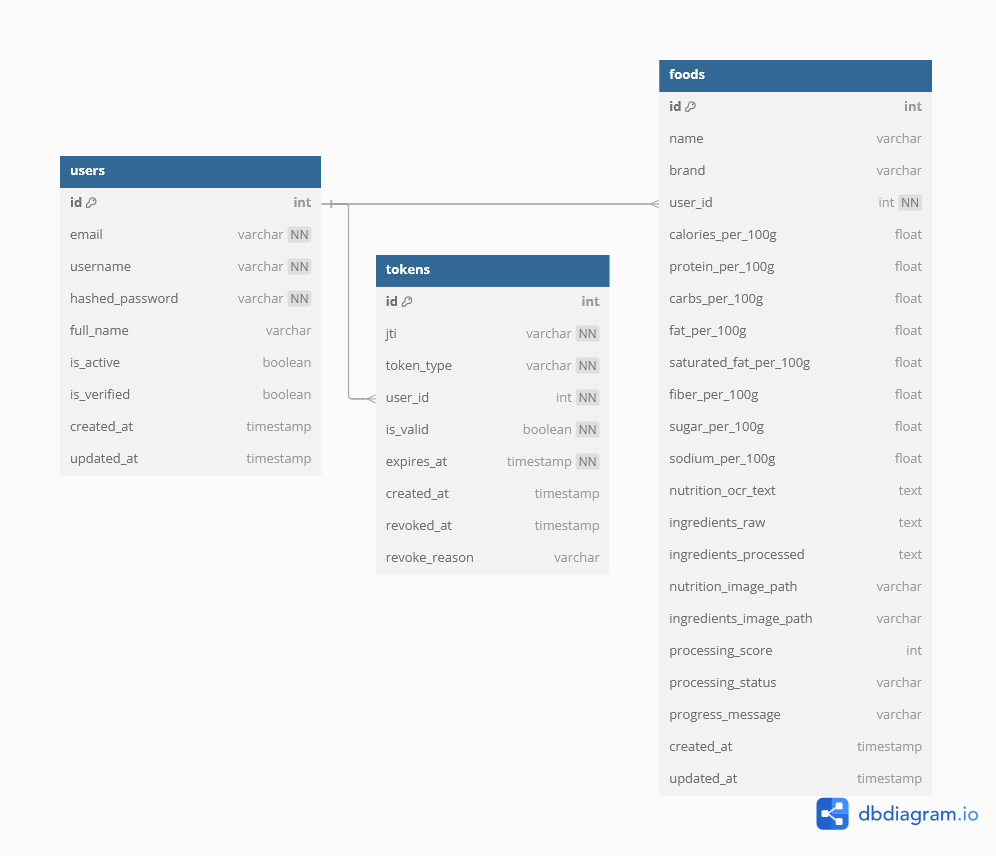
\includegraphics[width=0.9\textwidth]{images/db_diagram.png}
    \caption{Diagrama bazei de date, ilustrând relațiile dintre entitățile principale.}
    \label{fig:db-diagram}
\end{figure}